\section{16-bit Carry Look-ahead Adder(CLA) with Look Ahead Carry Unit}
\text{
$$ P[3:0] :- \textbf{Block Propagate Signal}$$
$$ G[3:0] :- \textbf{Generate Signal}$$
Now, by simultaneously calculating these queries, we may reduce the delay in the circuit rather than spreading out the carry out from one block to another. As a result, there is no need for successive blocks to wait for the carry from the prior one. As a result, the design becomes more modular and can calculate the Block Propagate and Generate Signals, which are useful when creating CLA Adders of Higher Order.}
\subsection{Circuit Diagram}
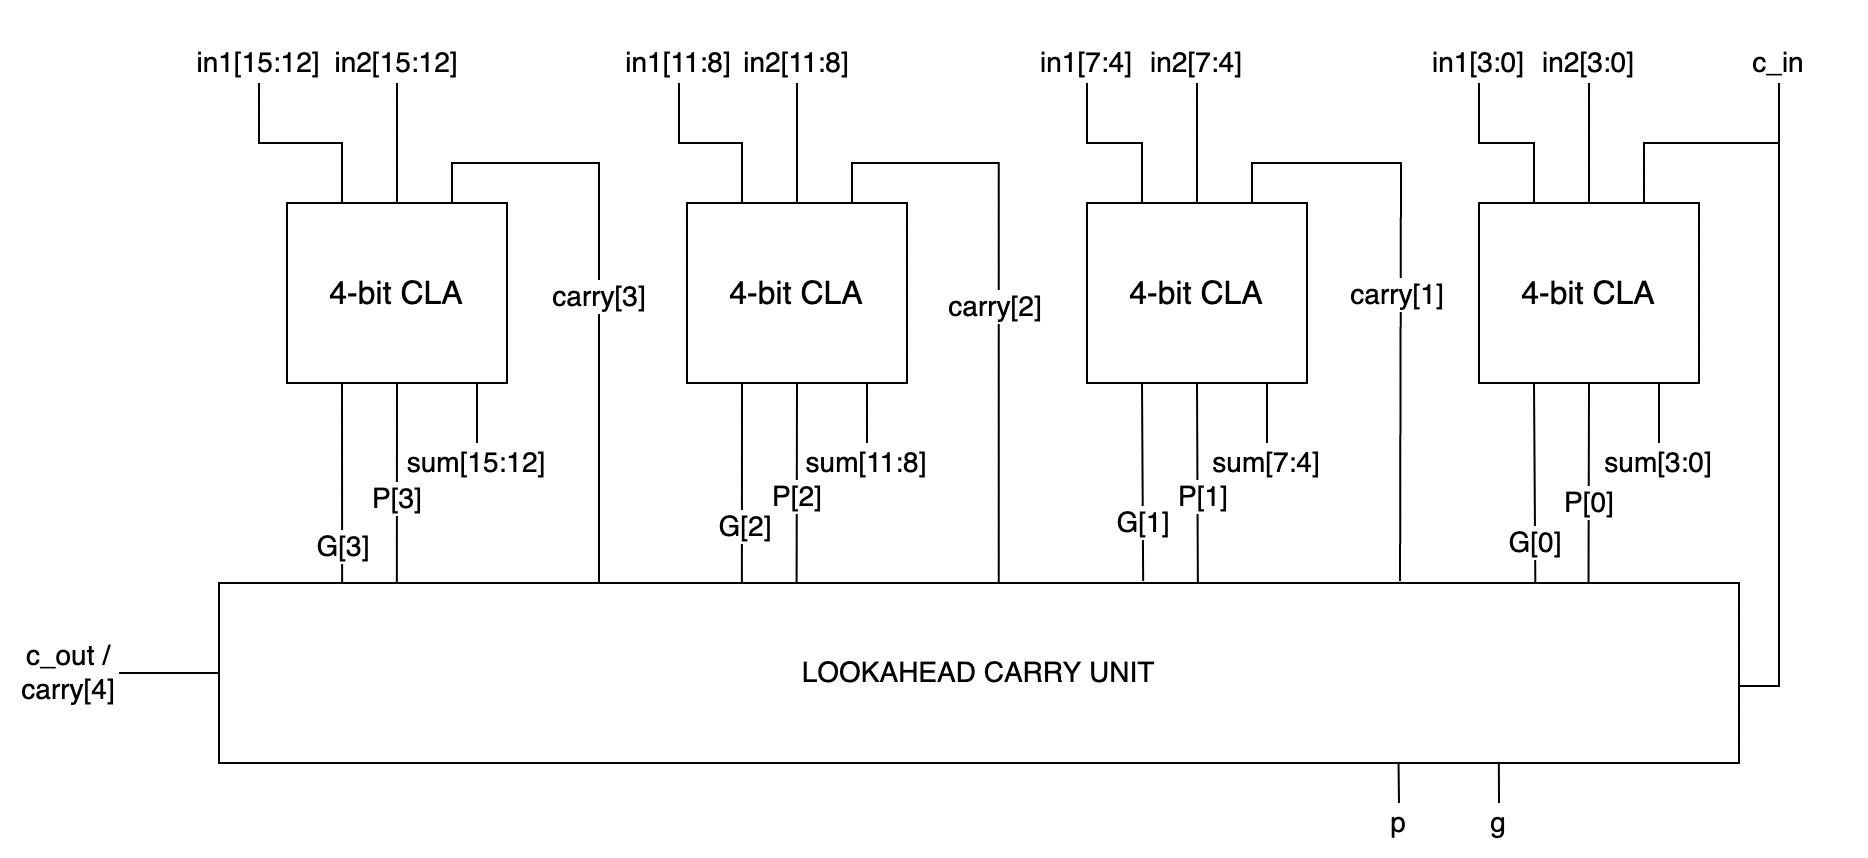
\includegraphics[width=18cm]{images/lca_16_lcu.png}
\subsection{Logic Expression}
The Logical Expressions for look-ahead carry unit are as follows:-
for P, G and C0,C1,.. C4 we can look upon the logical expressions enlisted in the 4-bit look-ahead carry adder.
for calculation of Block Propagate and Generate we have:-
\begin{equation} p = P[3] \And P[2] \And P[1] \And P[0]\end{equation}
\begin{equation} g = G[3] | (P[3] \And G[2]) | (P[3] \And P[2] \And G[1]) | (P[3] \And P[2] \And P[1] \And G[0]) )\end{equation}


